\documentclass[12pt, a4paper]{article}

% ── PAQUETES ─────────────────────────────────────────────────
% Los paquetes amplían las capacidades de LaTeX.
% Se cargan en el "preámbulo" (antes de \begin{document}).

\usepackage[utf8]{inputenc}       % Permite tildes y ñ
\usepackage[spanish]{babel}       % Idioma español (guiones, fechas, etc.)
\usepackage{geometry}             % Control de márgenes
\usepackage{graphicx}             % Para insertar imágenes
\usepackage{setspace}             % Control de interlineado
\usepackage{hyperref}             % Links clicables (índice, URLs)
\usepackage{xcolor}               % Colores personalizados
\usepackage{listings}
\usepackage{tcolorbox}
\usepackage{amsmath}
\usepackage{float}
\usepackage{booktabs}
\usepackage{subcaption}
\usepackage{chngcntr}
\usepackage{array}
\usepackage{tabularx}
\usepackage{ragged2e}

\counterwithin{figure}{subsection}
\tcbuselibrary{listings, skins}

\newtcblisting{terminal}{
    colback   = black,           % fondo negro
    colframe  = gray!50,         % borde gris
    coltitle  = black,           % título en blanco
    coltext   = green!70!white,  % texto verde (estilo terminal clásica)
    title     = Terminal,
    fonttitle = \bfseries\small,
    listing only,
    listing options = {
        basicstyle = \ttfamily\small\color{green!70!white},
        breaklines = true,
    }
}

\lstset{
    basicstyle    = \ttfamily\small,   % fuente monoespaciada
    keywordstyle  = \color{blue},      % palabras clave en azul
    commentstyle  = \color{gray},      % comentarios en gris
    stringstyle   = \color{orange},    % strings en naranja
    numbers       = left,              % números de línea a la izquierda
    frame         = single,            % recuadro alrededor del bloque
    breaklines    = true,              % corta líneas largas automáticamente
}

\newcommand{\tema}{Sistemas de comunicaciones básico}
\newcommand{\titulotrabajo}{Informe}
\newcommand{\autor}{Alfici, Facundo Ezequiel}
\newcommand{\documento}{44012327}
\newcommand{\curso}{PROCOM}
\newcommand{\fundacion}{Fundación Fulgor}
\newcommand{\fecha}{\today}

% ── INICIO DEL DOCUMENTO ─────────────────────────────────────
% Todo lo visible va DENTRO de este entorno
\begin{document}

% Quitamos la numeración en la carátula
\thispagestyle{empty}

% ── CARÁTULA ─────────────────────────────────────────────────
\begin{center}   % Entorno para centrar contenido

    % --- Encabezado institucional ---
    {\Large \textbf{\fundacion}}\\[0.3cm]      % \\ fuerza un salto de línea                 % [0.2cm] = espacio extra después
    {\large \curso}

    \vspace{1.5cm}   % Espacio vertical de 1.5 cm

    % --- Logo (opcional) ---
    % Descomenta las 2 líneas siguientes si tenés un logo guardado
    % \includegraphics[width=0.25\textwidth]{logo.png}
    % \vspace{1cm}

    \hrule height 1pt   % Línea horizontal
    \vspace{0.4cm}

    % --- Título del trabajo ---
    {\LARGE \textbf{\titulotrabajo}}\\[0.3cm]
    {\large \tema}

    \vspace{0.4cm}
    \hrule height 1pt

    \vspace{2.5cm}

    % --- Datos del alumno ---
    % Tabla simple de 2 columnas: etiqueta y valor
    \begin{tabular}{r l}   % r = columna alineada a la derecha, l = izquierda
        \textbf{Autor:}   & \autor\\[0.2cm]
        \textbf{Documento:}  & \documento\\[0.2cm]
        \textbf{Docentes:} &  Ariel Pola, Santiago Garaventta Pascual y Agustín Pesce\\
    \end{tabular}

    \vspace{3cm}

    % --- Fecha ---
    {\large \fecha}

\end{center}

% Salto de página → el informe real comienza en la siguiente hoja
\newpage

% ── EJEMPLO DE PRIMERA SECCIÓN (para no dejar el doc vacío) ──
\tableofcontents   % Genera el índice automáticamente
\newpage


\section{Introducción}
En este informe se aplicarán conceptos de los sistemas de comunicación vistos durante las clases,
con el fin de diseñar e implementar un sistema de comunicaciones básico, que consta de un PRBS de 9 bits,
un filtro RC y un contador de BER.

El trabajo consta de 4 partes;
\begin{enumerate}
    \item Diseño en Python de un simulador en punto flotante.
    \item Diseño en Python de un simulador en punto fijo, utilizando la librería \textbf{fixedInt.py} para la cuantización.
    Teniendo en cuenta además algunos conceptos de diseño de hardware y metodologías de retardo.
    \item Implementación en Verilog utilizando punto fijo.
    \item Implementación en FPGA.
\end{enumerate}

El diagrama en bloques que representa al sistema completo es el siguiente;
\begin{figure}[H]
    \centering
    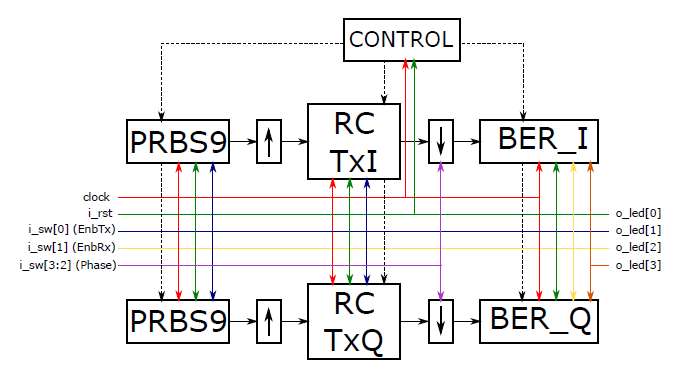
\includegraphics[width=1\textwidth]{imagenes/sist_comms.png}
    \caption{Diagrama en bloques del sistema de comunicaciones.}
    \label{fig:sist_comms}
\end{figure}

\newpage

\section{Desarrollo}
    \subsection{Simulador de Punto flotante}
    Para este apartado, se pidió implementar un simulador en punto flotante que contemple
    todo el diseño en donde la representación de la PRBS9 es una secuencia aleatoria y la estimación
    de la BER es una comparación de vectores.
    En primera medida, se definió la arquitectura del sistema, de manera que la interconexión entre la PRBS9 y el filtro RC
    tendrá un upsampling de 4 (dado el oversampling), es decir, por cada muestra que sale de la PRBS9, entrarán 4 muestras al filtro.
    Ahora, como criterio de diseño, se tomó la decisión de utilizar un sistema de multiplexores que evitan las multiplicaciones por 0
    de los coeficientes del filtro con los símbolos enviados por la PRBS.
    
    Este bloque será manejado por un clock lento con período de 1/T/os, de tal manera que, para cada baudio se realizará una selección 
    de la multiplicación a realizar dependiendo si es 0 o 1.
    \begin{itemize}
        \item En caso de que el símbolo sea 0, el coeficiente correspondiente será multiplicado por 1 y enviado al acumulador.
        \item En caso de que el símbolo sea 1, el coeficiente correspondiente será multiplicado por -1 y enviado al acumulador.
    \end{itemize}
    De esta manera, se evitará realizar un mapeado costoso en términos computacionales, método que también se conoce como \textbf{filtro polifásico}.

    Como consiguiente, el módulo de filtrado contendrá un apartado de graficación, donde se espera ver:
    \begin{itemize}
        \item Bits transmitidos.
        \item Respuesta al impulso y frencuencia del filtro Tx.
        \item Salida y diagrama de ojo del filtro Tx.
        \item Diagrama de constelación a la salida del filtro Tx (por cada fase).
    \end{itemize}
    
    Por otro lado, el contador de BER constará de un slicer previo, donde se busca retomar la cantidad deseada de símbolos reales.
    Luego, se utilizará una PRBS9 de referencia, que contiene la misma semilla de generación que la PRBS9 de la etapa de transmisión.

    Finalmente, es importante destacar los módulos de control y decodificación, donde principalmente se mapea los bits de la entrada
    i\_sw, que contiene el enable de transmisión, de recepción y los bits de selección de fase.
    
    \subsubsection{Gráficos obtenidos}
        Lo que respecta a los bits transmitidos por el sistema, se puede ver en la siguiente figura el resultado
        del tratamiento realizado.
        \begin{figure}[H]
            \centering
            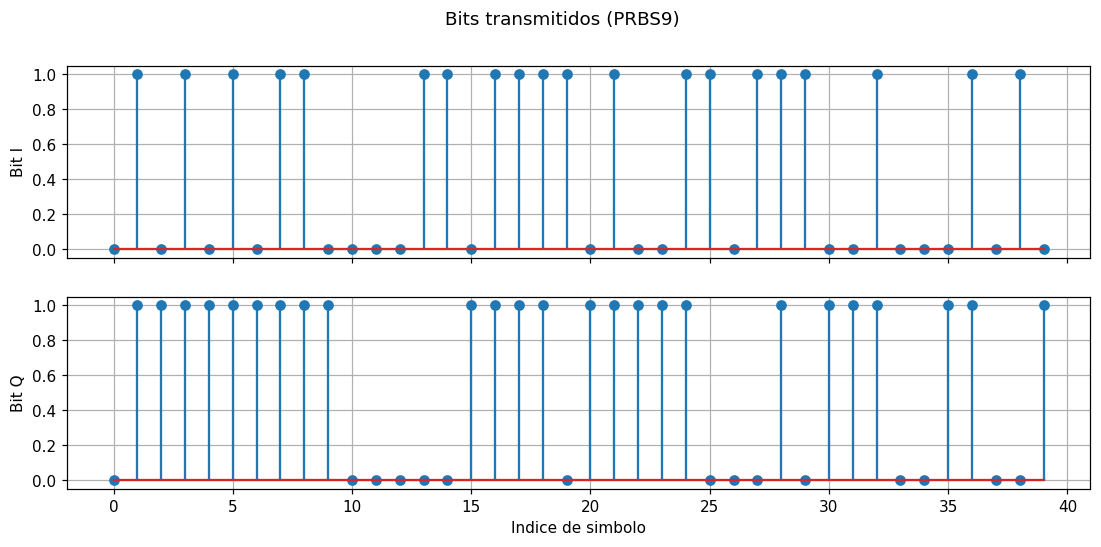
\includegraphics[width=1\textwidth]{imagenes/01_bits_transmitidos.png}
            \caption{Bits transmitidos en Fase(I) y Cuadratura(Q) respectivamente.}
            \label{fig:01_bits_transmitidos}
        \end{figure}
        De igual manera, se puede ver la respuesta al impulso y frecuencia del filtro Tx en la siguiente imagen.
        \begin{figure}[H]
            \centering
            \begin{subfigure}{0.49\textwidth}
                \centering
                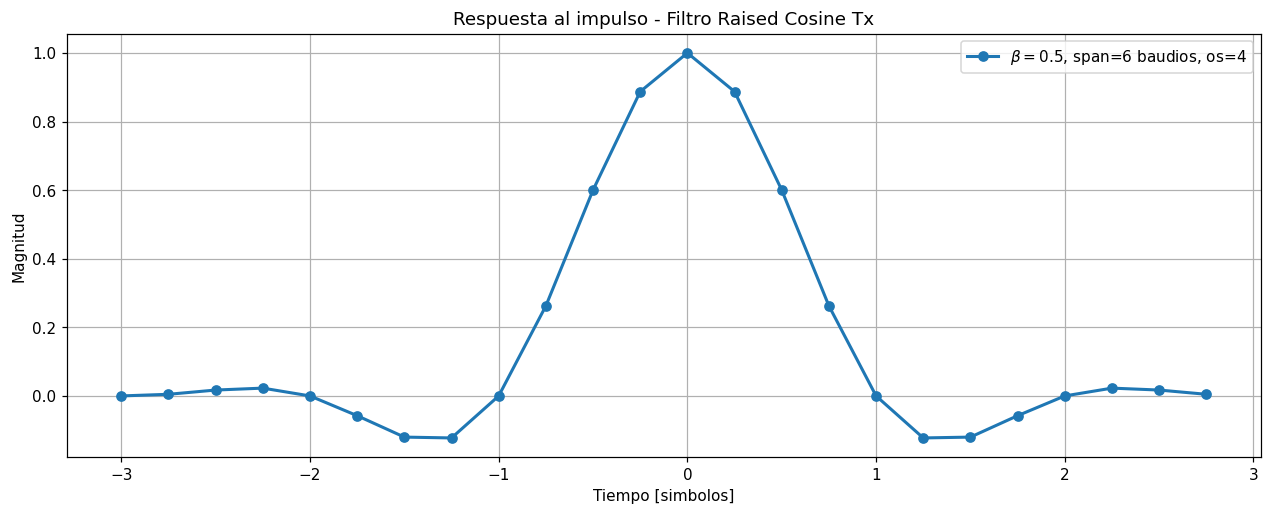
\includegraphics[width=\linewidth]{imagenes/02_respuesta_impulso.png}
            \end{subfigure}
            \hfill
            \begin{subfigure}{0.49\textwidth}
                \centering
                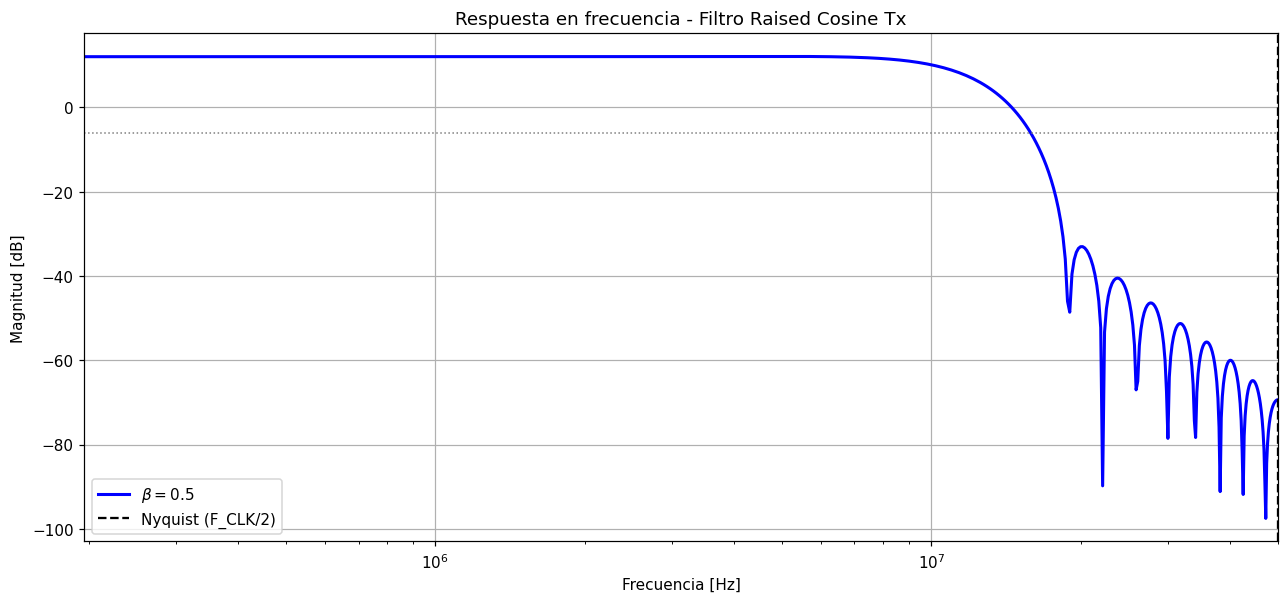
\includegraphics[width=\linewidth]{imagenes/03_respuesta_frecuencia.png}
            \end{subfigure}

            \caption{Respuesta al impulso y frecuencia del filtro Tx.}
            \label{fig:02_03_respuestas_tyf}
        \end{figure}
        
        En la figura \ref{fig:02_03_respuestas_tyf} se puede ver la naturaleza del filtro, donde la curva de respuesta al impulso
        tiene colas muy suavizadas y un valor normalizado a 1, como se pretendía.
        
        En lo que respecta a la salida del filtro polifásico, se tiene la siguiente imagen.
        \begin{figure}[H]
            \centering
            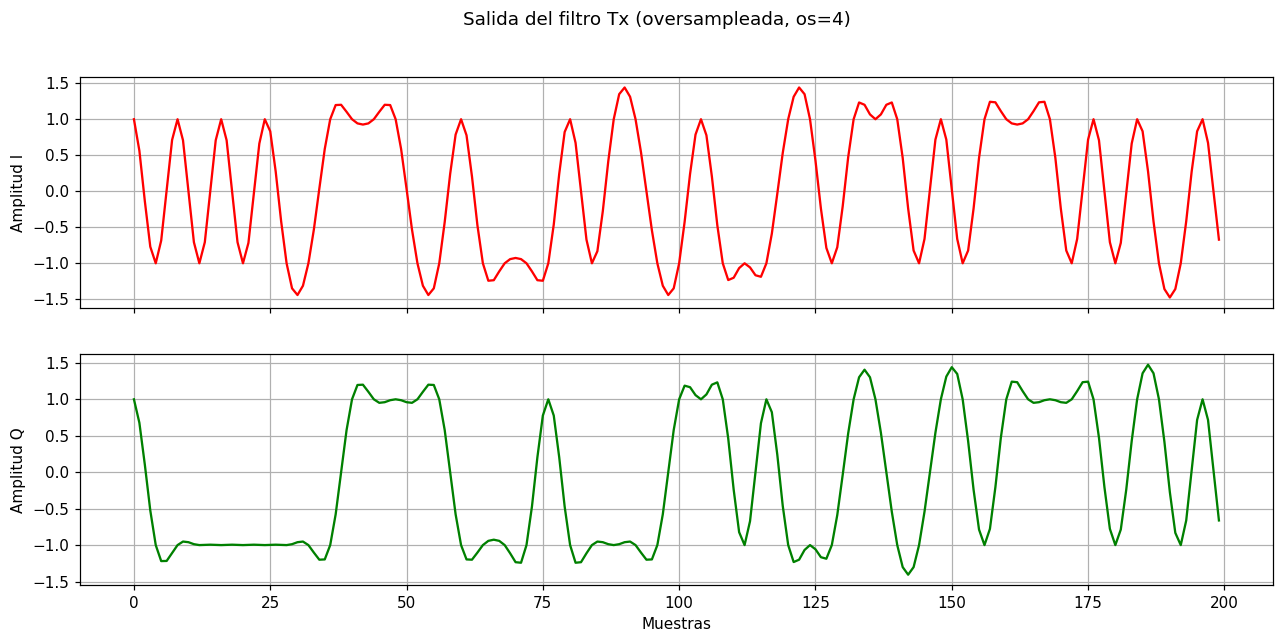
\includegraphics[width=1\textwidth]{imagenes/04_salida_filtro_tx.png}
            \caption{Salida del filtro polifásico en Fase(I) y Cuadratura(Q) respectivamente.}
            \label{fig:04_salida_filtro_tx}
        \end{figure}
        Esta imágen muestra los bits transmitidos ya filtrados, donde se pueden ver sobrepasamientos esperados
        en algunos de los símbolos, algo que será clave al momento de elegir la cuantización de los coeficientes del filtro.
        
        Finalmente, el diagrama de ojo y constelación por fase se puede ver a continuación.
        \begin{figure}[H]
            \centering
            \begin{subfigure}{0.49\textwidth}
                \centering
                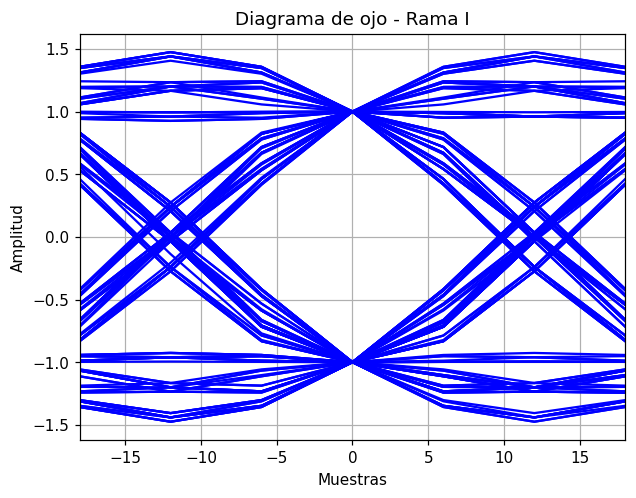
\includegraphics[width=\linewidth]{imagenes/05_ojo_I.png}
            \end{subfigure}
            \hfill
            \begin{subfigure}{0.49\textwidth}
                \centering
                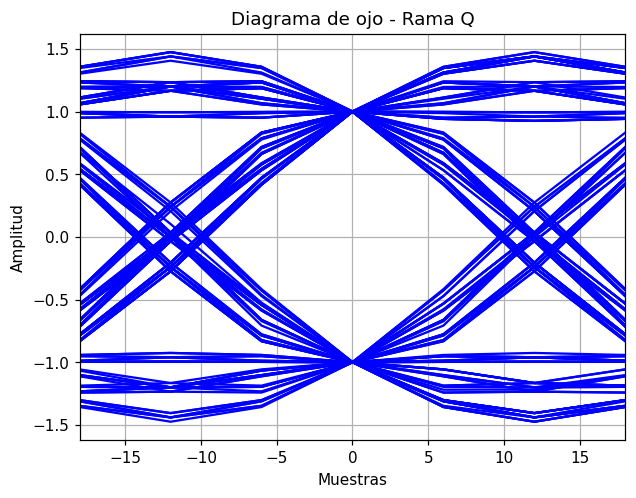
\includegraphics[width=\linewidth]{imagenes/06_ojo_Q.png}
            \end{subfigure}

            \caption{Diagrama de ojo de fase y cuadratura.}
            \label{fig:05_06_eye_diagram}
        \end{figure}
        \begin{figure}[H]
            \centering
            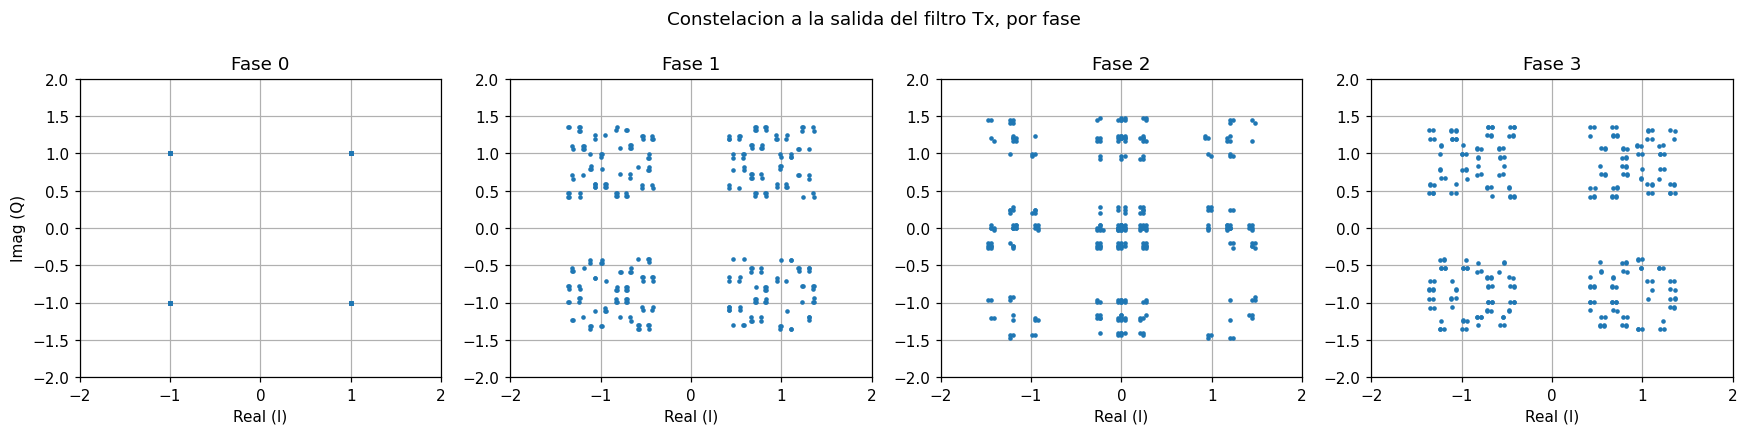
\includegraphics[width=1\textwidth]{imagenes/07_constelacion_por_fase.png}
            \caption{Constelaciones por fase float simulator.}
            \label{fig:07_constelacion_por_fase}
        \end{figure}
        Estas figuras muestran que, para la fase 0 se tiene una ISI nula, siendo ésta la fase óptima del filtro. Considerando un
        análisis mas detallado se concluye;
        \begin{itemize}
            \item La fase 0 se representa el símbolo transmitido correctamente.
            \item Las fases 1 y 3 presentan nubes de puntos alrededor de un punto medio, lo que tiene sentido 
            debido a que son las fases más cercanas a la fase 0.
            \item La fase 2 tiene errores por el cruce en los ejes del plano complejo.
        \end{itemize}    
        Este dato se puede corroborar utilizando el contador de BER, donde se muestra el Bit Error Rate para cada fase por 
        separado.
        \begin{figure}[H]
            \centering
            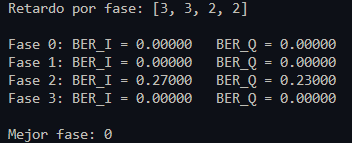
\includegraphics[width=1\textwidth]{imagenes/BER_float.png}
            \caption{BER de fase y cuadratura por cada fase.}
            \label{fig:BER_float}
        \end{figure}
        Algo a destacar es que existirá un retardo por fase introducido manualmente, esto se debe a que
        el cambio de fase adelanta el generador y genera un corrimiento de la lectura del bit actual, lo que se traduce a
        un BER elevado para las fases afectadas.
    
    \subsection{Simulador de Punto Fijo}
    Para este inciso se pide realizar algunos cambios de la arquitectura de manera tal
    que se parezca a una implementación en hardware, agregando también la cuantización en punto fijo.
    
    La selección de la cuantización óptima para este inciso fue S(9,7), debido a que, como ya se comentó antes,
    la salida del filtro generará picos que sobrepasarán el valor normalizado propuesto para el filtro.
    Por esta razón, se planteó lo siguiente:
    \begin{itemize}
        \item 1 bit de signo
        \item 1 bit de parte entera
        \item 7 bits de parte fraccionaria
    \end{itemize}
    De esta manera, se podrá representar cualquier valor que sobrepase el 1 y a la vez tener una buena resolución sin
    que haya mucha carga computacional.
    Lo mismo se planteó para la salida de los acumuladores que representan el filtro polifásico, habiendo así un forzamiento
    a S(9,7) tomando siempre las partes más significativas de las palabras y redondeando el resto.

    Lo que respecta al contador de BER, nuevamente se tomó lo planteado en el simulador de punto flotante, donde se utilizó
    una PRBS9 de referencia para la comparación de los bits recibidos.

    Sobre la metodología utilizada para los retardos del sistema, se utilizó una variable que representa el delay por símbolo,
    de tal manera que el desplazamiento del pico del filtro generado por la cuantización no será significante.
    \subsubsection{Gráficos obtenidos}
        \begin{figure}[H]
            \centering
            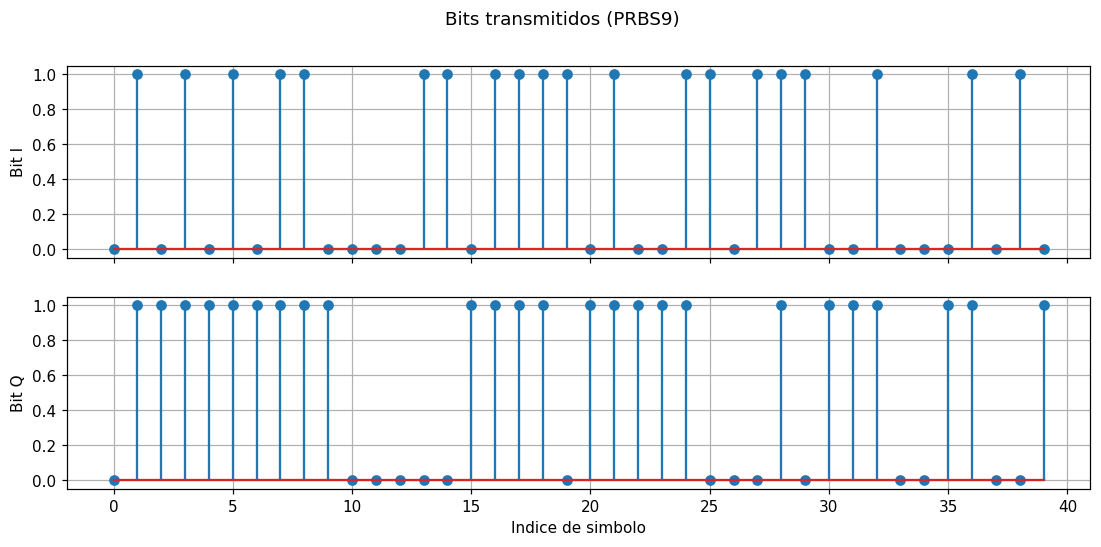
\includegraphics[width=1\textwidth]{imagenes/01_bits_transmitidos_fp.png}
            \caption{Bits transmitidos en Fase(I) y Cuadratura(Q) respectivamente.}
            \label{fig:01_bits_transmitidos_fp}
        \end{figure}
        De igual manera, se puede ver la respuesta al impulso y frecuencia del filtro Tx en la siguiente imagen.
        \begin{figure}[H]
            \centering
            \begin{subfigure}{0.49\textwidth}
                \centering
                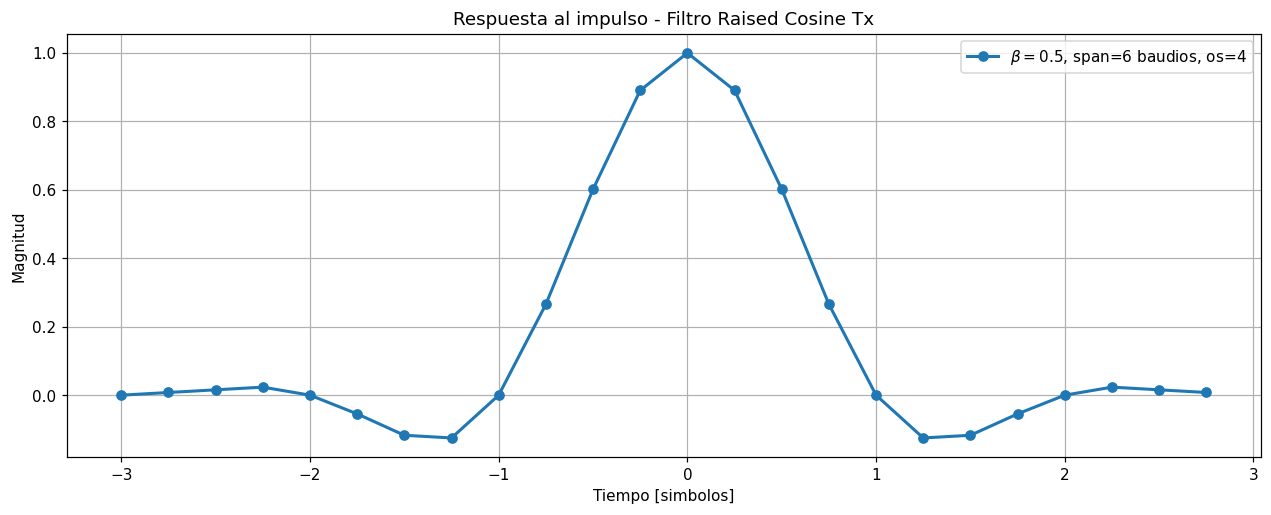
\includegraphics[width=\linewidth]{imagenes/02_respuesta_impulso_fp.png}
            \end{subfigure}
            \hfill
            \begin{subfigure}{0.49\textwidth}
                \centering
                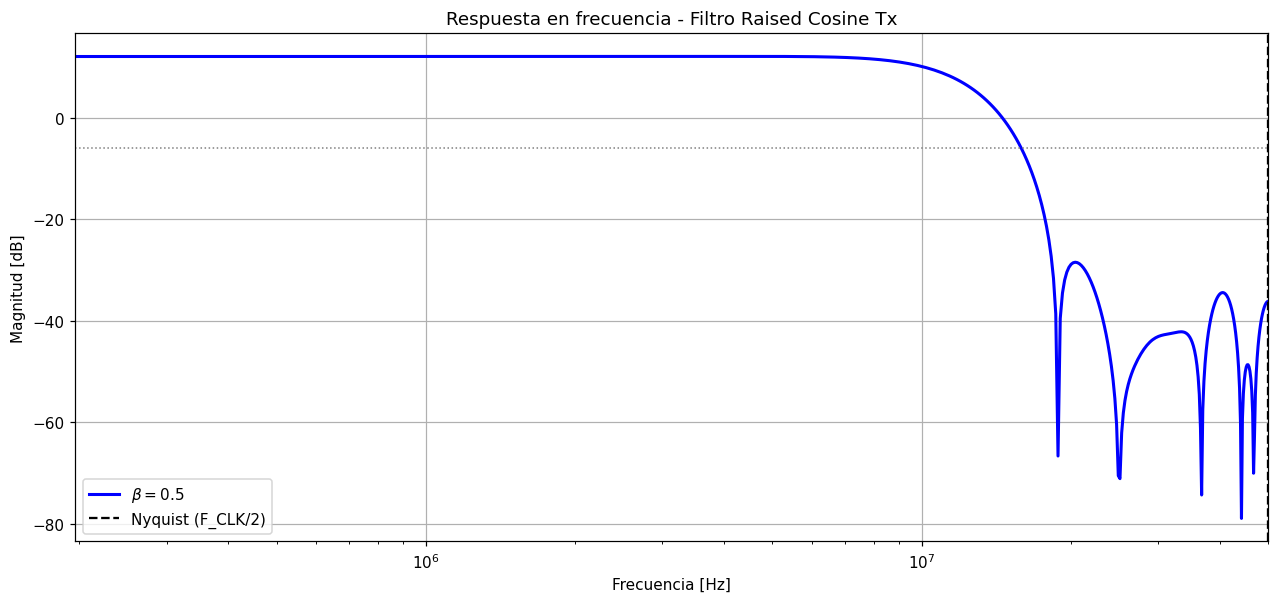
\includegraphics[width=\linewidth]{imagenes/03_respuesta_frecuencia_fp.png}
            \end{subfigure}

            \caption{Respuesta al impulso y frecuencia del filtro Tx con punto fijo.}
            \label{fig:02_03_respuestas_tyf_fp}
        \end{figure}
        
        La respuesta vista en la figura \ref{fig:02_03_respuestas_tyf_fp} nos dice que
        la representación de la salida no se verá afectada en mayor medida debido a la cuantización, por lo que podríamos
        esperar un resultado muy similar al obtenido en el modelo de punto flotante para los demás apartados.

        En lo que respecta a la salida del filtro polifásico, se tiene la siguiente imagen.
        \begin{figure}[H]
            \centering
            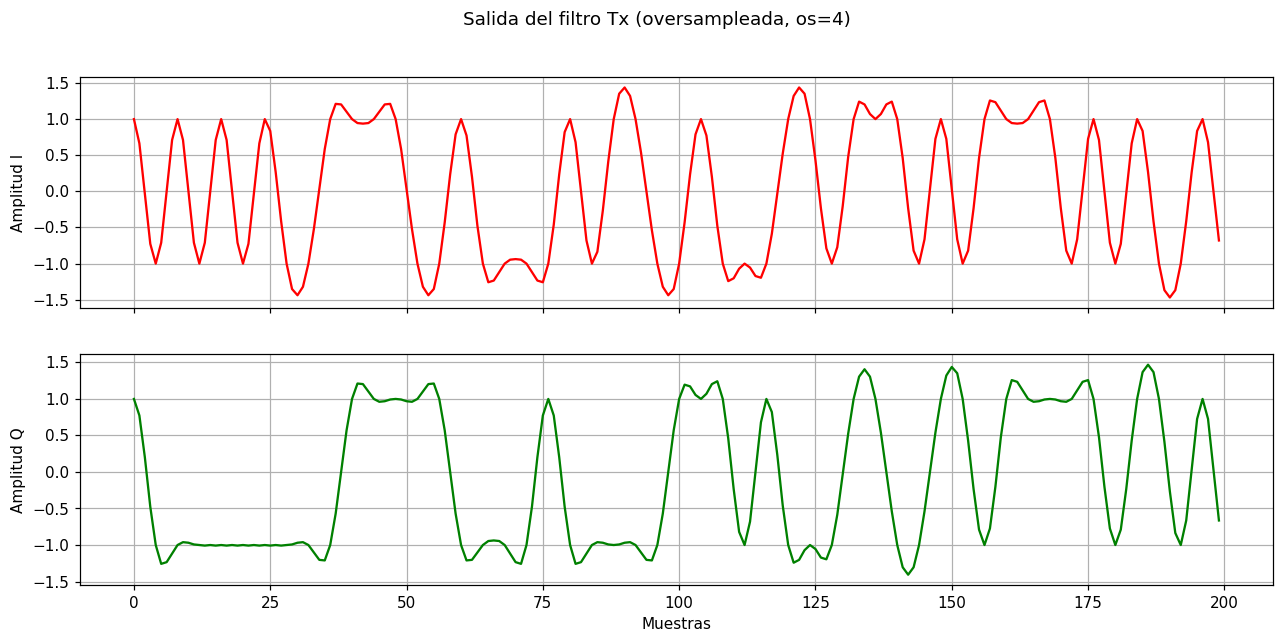
\includegraphics[width=1\textwidth]{imagenes/04_salida_filtro_tx_fp.png}
            \caption{Salida del filtro polifásico en Fase(I) y Cuadratura(Q) en punto fijo.}
            \label{fig:04_salida_filtro_tx_fp}
        \end{figure}
        Comparado el resultado obtenido con la figura \ref{fig:04_salida_filtro_tx} se puede ver que
        la representación de los símbolos es muy fiel.

        Finalmente, el diagrama de ojo y constelación por fase se puede ver a continuación.
        \begin{figure}[H]
            \centering
            \begin{subfigure}{0.49\textwidth}
                \centering
                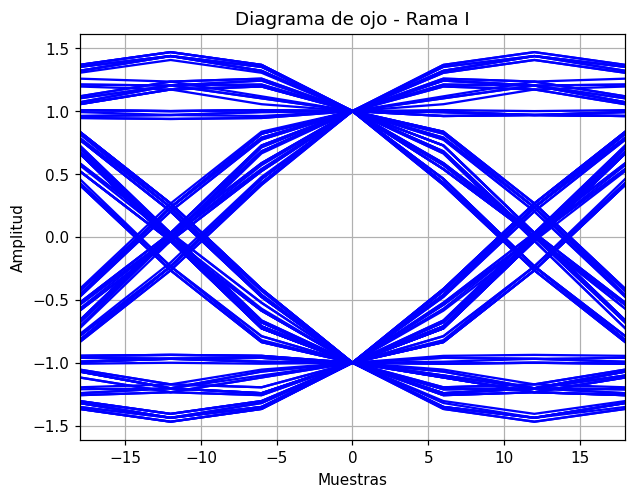
\includegraphics[width=\linewidth]{imagenes/05_ojo_I_fp.png}
            \end{subfigure}
            \hfill
            \begin{subfigure}{0.49\textwidth}
                \centering
                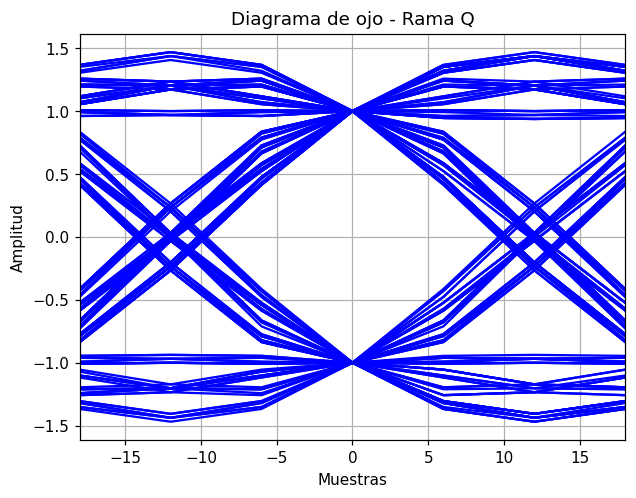
\includegraphics[width=\linewidth]{imagenes/06_ojo_Q_fp.png}
            \end{subfigure}

            \caption{Diagrama de ojo de fase y cuadratura en punto flotante.}
            \label{fig:05_06_eye_diagram_fp}
        \end{figure}
        \begin{figure}[H]
            \centering
            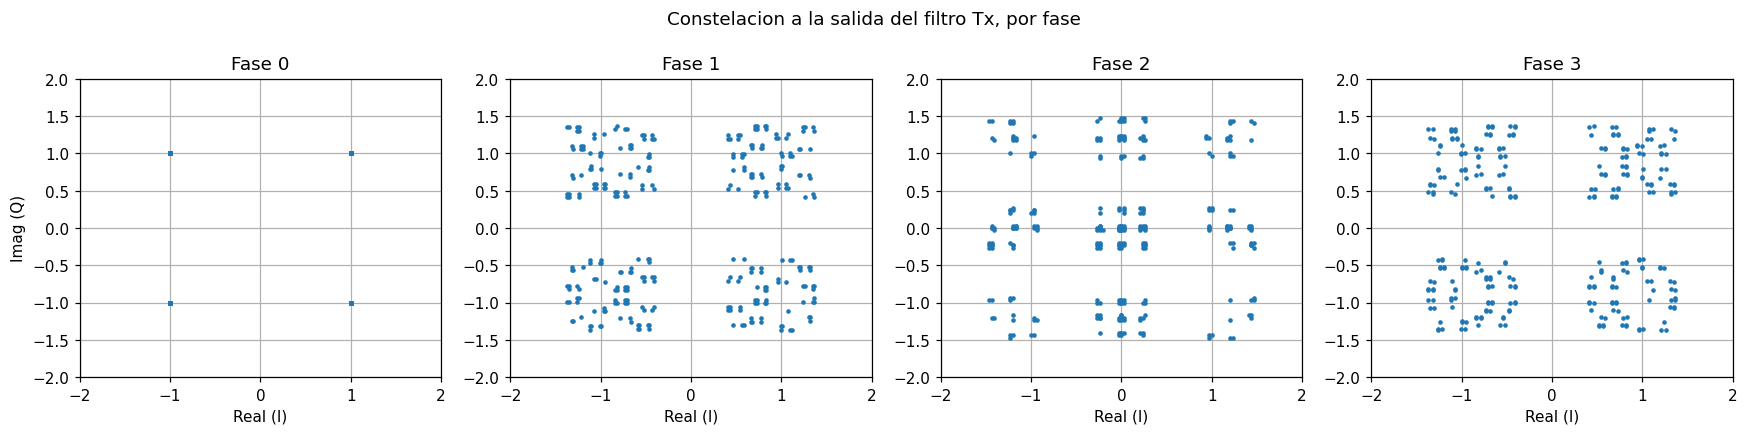
\includegraphics[width=1\textwidth]{imagenes/07_constelacion_por_fase_fp.png}
            \caption{Constelaciones por fase fixed point simulator.}
            \label{fig:07_constelacion_por_fase_fp}
        \end{figure}
        Lo visto demuestra que, el simulador de punto fijo con arquitectura de hardware real se comporta correctamente,
        dando resultados prácticamente iguales a los obtenidos en el simulador de punto flotante, como se muestra en la figura \ref{fig:07_constelacion_por_fase}
        \begin{figure}[H]
            \centering
            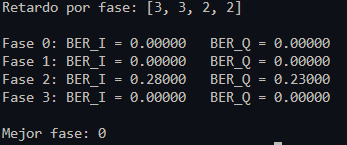
\includegraphics[width=1\textwidth]{imagenes/BER_fp.png}
            \caption{BER de fase y cuadratura por cada fase de punto flotante.}
            \label{fig:BER_fp}
        \end{figure}
    \subsection{Implentación en Verilog del modelo en punto fijo.}
        En este inciso, se desarollará el modelo en punto fijo en Verilog, previamente propuesto en Python.
        Siendo un lenguaje donde se pretende desarrollar el programa de la forma más prolija posible, se dividirá el código en bloques
        funcionales para cada etapa.
        \subsubsection{}
\end{document}